
\documentclass[12pt]{article}
\usepackage{graphicx}
\usepackage{amsmath}
\usepackage{listings}
\usepackage{color}
\usepackage{float}

\definecolor{dkgreen}{rgb}{0,0.6,0}
\definecolor{dkblue}{rgb}{0,0.0,0.6}
\definecolor{dkred}{rgb}{0.9,0.0,0.1}

\begin{document}

\lstset{language=Fortran,tabsize=4,numbers=left,numberstyle=\tiny,basicstyle=\ttfamily\small\color{dkblue},stringstyle=\ttfamily\color{blue},keywordstyle=\rmfamily\color{dkred}\bfseries\emph,backgroundcolor=\color{white},commentstyle=\color{dkgreen}}

\title{Midterm 1}
\author{Paul Fischer \\
Department of Physics\\
California State University Long Beach}
\date{\today }

\maketitle

\begin{abstract}

The Runge-Kutta method RK4 is used to study a double pendulum (Problem 1) and a vibrating neutron star (Problem 2).  We analyze the energies of the double pendulum for four different sets of initial conditions and observe their corresponding Poincare sections.  We observe that a vibrating neutron star will have a nearly constant z-component while also nutating about the z-axis.

\end{abstract}

\section{Introduction}

Ever since Newton's 2$^{nd}$ Law was published, Physics has been formulated in the language of differential equations.  Many nonlinear ordinary differential equations that arise in physics have no analytical solutions in terms of elementary functions.  Physicists often use numerical approximation methods to simulate such systems.  Around the year 1900, Mathematicians Carl Runge and Wilhelm Kutta developed a series of implicit and explicit iterative methods for approximating solutions to ordinary differential equations \cite{wiki}.  At each iteration, the method uses a trial step in the middle of a determined interval to cancel lower-order terms.  The code we will use takes advantage of the RK4 method, which is a fourth-order formula which is shown below \cite{weisstein}:

\[k_1 = h f(x_n, y_n)\]
\[k_2 = h f(x_n + \frac{1}{2} h, y_n + \frac{1}{2} k_1)\]
\[k_3 = h f(x_n + \frac{1}{2} h, y_n + \frac{1}{2} k_2)\]
\[k_4 = h f(x_n + h, y_n + k_3)\]
\[y_{n+1} = y_n + \frac{1}{6} k_1 + \frac{1}{3} k_2 + \frac{1}{3} k_3 + \frac{1}{6} k_4 + O(h^5)\]

This midterm will be organized as follows.  In section Problem 1 (Analysis), the answers to Problem 1 will be discussed qualitatively, followed by the code in section Problem 1 (Code) and the figures in the section Problem 1 (Figures).  The length of the code and number of figures required for Problem 1 have warranted them getting their own sections.  Section Problem 2 contains an analysis of the vibrating neutron star simulation.  This will be followed by the Summary and Conclusions section.  

\section{Problem 1 (Analysis)}

For the first problem we are asked to solve the problem of the double pendulum using the \emph{rk4} method.  This is done using the subroutine {\tt rk4step}.  We create an array $y = (\theta_1, \omega_1, \theta_2, \omega_2)$ and insert parameters $g = 1$, $l_1 = 2$, $m_1 = 3$, $l_2 = 1$, and $m_2 = 1$.  We must first determine the energies for different initial conditions, namely $E_1(0,0,0,0)$, $E_2(\pi,0,0,0)$, $E_3(0,0,\pi,0)$, and $E_4(\pi,0,\pi,0)$. To determine the energy of the system given the initial conditions, we must derive its kinetic and potential energies in plane-polar coordinates.  We start with the parametrization of $(x_1, y_1, x_2, y_2)$ in terms of $\theta_1$ and $\theta_2$, \textbf{where we set the resting position of $m_2$ as $(x_2, y_2) = (0, 0)$} (this is a personal choice, not a necessary one):

\[x_1 = l_1 sin \theta_1\]
\[y_1 = l_2 + l_1(1 - cos \theta_1)\]
\[x_2 = l_1 sin \theta_1 + l_2 sin \theta_2\]
\[y_2 = l_1(1 - cos \theta_1) + l_2(1 - cos \theta_2)\]

We plug this parametrization into the kinetic and potential energies for the system:

\begin{align*}
    T &= \frac{1}{2} m_1 (\dot{x}_1^2 + \dot{y}_1^2) + \frac{1}{2} m_2 (\dot{x}_2^2 + \dot{y}_2^2)\\
      &= \frac{1}{2} (m_1 + m_2) l_1^2 \omega_1^2 + \frac{1}{2} m_2 l_2^2 \omega^2 + m_2 l_1 l_2 \omega_1 \omega_2 cos (\theta_1 - \theta_2)
\end{align*}

\begin{align*}
    V &= m_1 g y_1 + m_2 g y_2\\
      &= m_1 g l_2 + (m_1 + m_2) g l_1 (1 - cos \theta_1) + m_2 g l_2 (1 - cos \theta_2)
\end{align*}

This reveals a Lagrangian:

\begin{align*}
    \mathcal{L} &= T - V\\
      &= \frac{1}{2} (m_1 + m_2) l_1^2 \omega_1^2 + \frac{1}{2} m_2 l_2^2 \omega^2 + m_2 l_1 l_2 \omega_1 \omega_2 cos (\theta_1 - \theta_2)\\ 
      &\;\;\;\;\;- m_1 g l_2 - (m_1 + m_2) g l_1 (1 - cos \theta_1) - m_2 g l_2 (1 - cos \theta_2).
\end{align*}

We can solve for the equations of motion using the Euler-Lagrange equations:

\[\frac{d}{dt} \frac{\partial \mathcal{L}}{\partial \dot{q}} - \frac{\partial \mathcal{L}}{\partial q} = 0\].

For $q \in [\theta_1,\theta_2]$, $\dot{q} \in [\omega_1, \omega_2]$ we obtain the equations of motion:

\[\dot{\omega}_1 = \frac{-m_2 l_2 [\dot{\omega}_2 cos(\theta_1 - \theta_2) + w_2^2 sin(\theta_1 - \theta_2)] - (m_1 + m_2) g sin \theta_1}{(m_1+m_2)l_1}\]

\[\dot{\omega_2} = - \frac{1}{l_2} (l_1[\dot{\omega_1} cos(\theta_1 - \theta_2) - \omega_1^2 sin(\theta_1 - \theta_2)] + g sin \theta_1)\].

For rk4, the differential equations must be uncoupled so they can be rearranged through the a substitution that will produce the following results \cite{neumann}.  We use the following variables to represent the method rk4 in our code:

\[y(1) = \theta_1\]
\[f(1) = y(2) = \dot{\theta_1} = \omega_1\]
\begin{align*}
    f(2) &= \dot{\omega_1} \\
    &= \frac{-g(2m_1+m_2)sin\theta_1-m_2gsin(\theta_1-2\theta_2)}{l_1(2m_1+m_2-m_2cos(2\theta_1-2\theta_2))} \\
    &\;\;\;\;\;\frac{-2sin(\theta_1-\theta_2)m_2(\omega_2^2l_2+\omega_1^2l_1cos(\theta_1-\theta_2))}{l_1(2m_1+m_2-m_2cos(2\theta_1-2\theta_2))}
\end{align*}
\[y(3) = \theta_2\]
\[f(3) = y(4) = \dot{\theta_2} = \omega_2\]
\begin{small}
\begin{align*}
    f(4) &= \dot{\omega_2} \\
    &= \frac{2sin(\theta_1-\theta_2)(\omega_1^2l_1(m_1+m_2)+g(m_1+m_2)cos\theta_1+\omega_2^2l_2m_2cos(\theta_1-\theta_2))}{l_2(2m_1+m_2-m_2cos(2\theta_1-2\theta_2))}
\end{align*}
\end{small}

The total energy, $E$, is the sum of the kinetic energy, $T$, and potential energy, $V$, which were derived above.  When using this model for the double pendulum, we assume the system is closed and that therefore the energy will be conserved.  This means we only need to calculate the energy at the initial conditions to have the value for the energy of the system at all times.  We can notice that for all four given initial conditions, $\omega_1 = 0$.  This means that before calculating the energy directly in our {\tt Fortran90} code we can simplify the calculation.  Plugging in this condition reveals the following expression for the energy:

\[E_i = \frac{1}{2} m_2 l_2^2 \omega_2^2 + g[m_1(l_2+l_1[1-cos\theta_1])+m_2 g(l_1[1-cos\theta_1]+l_2[1-cos\theta_2])]\]

Plugging the initial conditions into this expression for calculating and using it to calculate the energies in the {\tt Fortran90} code reveals the values:

\[E_1(0,0,0,0)=3\]
\[E_2(0,0,\pi,0)=5\]
\[E_3(\pi,0,0,0)=19\]
\[E_4(\pi,0,\pi,0)=21\]

\textbf{These values can be shifted based on where the position $y=0$ is set for the potential energy, these values come from setting the resting position of $m_2$ at $(x,y)=(0,0)$, setting the pivot point for the first pendulum as the $y=0$ would result in energies $E_i \in [-9, -7, 7, 9]$, $i \in [1, 2, 3, 4]$.}

By noticing that $\omega_2=0$ in all of these initial conditions as well, the $E_i$ term will cancel out all of the terms to the right of the $\omega_2$ term in the $E_i$ equation given above.  Therefore, we can calculate the value of $\omega_2$ in the code with the folowing expression:

\[\omega_2=\frac{2 \Delta E}{m_2 l_1^2}\]

We can notice that this equation is independent of the energies, so for all given initial conditions the $\omega_2$ such that $E=E_i+\Delta E$, $i \in [1,2,3,4]$ will reveal the following value calculated by the {\tt Fortran90} code:

\[\omega_2=0.14142135465680267\]

The code is shown in the following section.  The Makefile is shown in Listing \ref{makefile} and it contains flags to optimize th calculation and shows that we can run the code by typing {\tt pen} into the terminal after it has been compiled by typing {\tt make}.  Listing \ref{numtype} contains the {\tt numtype} file, which defines the precision of the values we will use as well as our value of {\tt pi}.  The file {\tt dubpen.f90} is found in Listing \ref{dubpen} and begins with the module {\tt setup} which defines the parameters and the length of the arrays for {\tt y} and {\tt f} required by rk4.  The program begins with defining the initial conditions and time parameters.  The code here has the initial conditions for energy $E_4$ and shows that we are simulating for a time of 600 s with a step {\tt dt = 0.1}.  Then we calculate and print out the initial energy and $\omega_2$ value required by the problem.  The do-loop first plots the angles $\theta_1$ and $\theta_2$ as functions of time as the files {\tt fort.1} and {\tt fort.2}.  A section to plot energy as a function of time was placed in the do loop to see if rk4 would conserve total energy, which should happen in this model with this closed system.  Then the Poincare section is plotted, which is a graph of the values of $\omega_2$ vs. $\theta_2$ at each time where $\theta_1=0$ and $\omega_1>0$.  Since this code is a numerical approximation, the Poincare section of the code bounds the angles $\theta_1$ and $\theta_2$ to be in the range $[-\pi,\pi)$ and looks for when $\theta_1 \in (-0.1,0.1)$.  To calculate the values of $\theta_1$ and $\theta_2$ at each iteration of the do-loop, the function {\tt rk4step} is called on.  The {\tt y} and {\tt f} arrays are defined as above.  Fig. \ref{th2vte1}, \ref{th2vte1}, \ref{pse1}, and \ref{evte1} shown in section Problem 1 (Figures) represent the results of the code for the initial conditions set for $E_1$.  All of the graphs are made with giving the initial energy that small boost in $\omega_2$ calculated earlier.  Since the system starts nearly at rest in $E_1$, the behavior is similar to a regular pendulum, and the graphs appear to be periodic and the Poincare section is fairly symmetric.  The energy as a function of time changes by approximately 1\%, so it is not conserved with rk4 but stays close enough to being conserved to represent a fairly accurate simulation.  Fig. \ref{th1vte2}, \ref{th2vte2} and \ref{pse3} are for the initial conditions given for $E_2$.  This still involves no initial angle given for $\theta_1$, so the motion is still similar to a single pendulum and not chaotic, giving a periodic graph for $\theta_1$ and another well-behaved Poincare section.  However, this extra energy allows us to see some behavior that creates some chaos as we see $\theta_2$ start to cycle around different values.  Fig. \ref{th1vte3}, \ref{th2vte3}, \ref{pse3} are for $E_3$ and Fig. \ref{th1vte4}, \ref{th2vte4} and \ref{pse4} are for $E_4$.  The graphs for these two initial conditions start with a significant $\theta_1$ value so the behavior is not periodic and chaotic.  The spatial graph for $E_3$ shown in Fig. \ref{yvxe3} was made to visually represent the spatial path of the masses in the double pendulum and it acts as a check that the code is working properly.

\section{Problem 1 (Code)}

\begin{lstlisting}[frame=single,caption={{\tt Makefile}},label=makefile]

objs1 = numtype.o dubpen.o 

prog1 = pen

f90 = gfortran

f90flags = -O3 

libs = -framework Accelerate

ldflags = $(libs)

all: $(prog1)

$(prog1): $(objs1)
	$(f90) $(ldflags) -o $@ $(objs1)

clean: 
	rm -f $(prog1) *.{o,mod} fort.*

.suffixes: $(suffixes) .f90

%.o: %.f90
	$(f90) $(f90flags) -c $<

\end{lstlisting}

\begin{lstlisting}[frame=single,caption={Module {\tt numtype}},label=numtype]

module numtype

    save
    integer, parameter :: &
        dp = selected_real_kind(15,307)
    real(dp), parameter :: pi = 4*atan(1._dp)

end module numtype

\end{lstlisting}

\begin{lstlisting}[frame=single,caption={The Program {\tt dubpen.f90}.},label=dubpen]

module setup

    use numtype
    implicit none
    integer, parameter :: n_eq = 4

    real(dp), parameter :: g = 1._dp, l_1 = 2._dp, &
        m_1 = 3._dp, l_2 = 1._dp, m_2 = 1._dp

end module setup

program dubpen

    use setup
    implicit none
    real(dp), dimension(n_eq) :: y
    real(dp) :: t, dt, tmax, w2, y1, yl, yu, &
        x_1, x_2, y_1, y_2, E, Et, eps, y3
    real(dp), dimension(3) :: Ei
    real(dp), dimension(4) :: Ef

    t = 0._dp
    dt = 0.1_dp
    tmax = 600._dp

    ! Enter initial conditions
    y(1) = pi                  ! theta_1
    y(2) = 0._dp               ! omega_1
    y(3) = pi                  ! theta_2
    y(4) = 0.14142135465680267 ! omega_2

    ! Energy terms to be summed
    Ei(1) = 1._dp / 2 * m_2 * l_2**2 * y(4)**2
    Ei(2) = m_1 * g * ( l_2 + l_1 &
        & * ( 1 - cos( y(1) ) ) )
    Ei(3) = m_2 * g * ( l_1 * ( 1 - cos( y(1) ) ) &
        & + l_2 * ( 1 - cos( y(3) ) ) )

    ! Energy for intial conditions
    E = sum( Ei )

    ! w2 such that E = Ei + 0.01
    w2 = sqrt( 2 * ( 0.01 ) / ( m_2 * l_2**2 ) )

    print *, "E =", E, "w2 =", w2

    ! For plotting Poincare section
    eps = 0.2

    do while ( t < tmax )


        ! Plot angles vs. time
        write(1,*) t, y(1)
        write(2,*) t, y(3) 

        ! Plot positions y vs. x
        x_1 = l_1 * sin( y(1) )
        y_1 = l_2 + l_1 * ( 1 - cos( y(1) ) )
        x_2 = x_1 + l_2 * sin( y(3) )
        y_2 = y_1 - l_2 * cos( y(3) )
        write(3,*) x_1, y_1 
        write(4,*) x_2, y_2 

        ! Plot energy vs. time
        Ef(1) = 1._dp / 2 * ( m_1 + m_2 ) &
            & * l_1**2 * y(2)**2
        Ef(2) = 1._dp / 2 * m_2 * l_2**2 * y(4)**2
        Ef(3) = m_2 * l_1 * l_2 * y(2) &
            & * y(4) * cos( y(1) - y(3) )
        Ef(4) = m_1 * g * ( y_1 + y_2 )
        Et = sum( Ef )
        write(7,*) t, Et

        ! Plot Poincare Section
        y1 = y(1)
        y3 = y(3)
        if ( y1 >= pi ) then
            do while ( y1 >= pi )
                y1 = y1 - 2 * pi
            end do
        elseif ( y1 < - pi ) then
            do while ( y1 < - pi )
                y1 = y1 + 2 * pi
            end do
        end if
        if ( y3 >= pi ) then
            do while ( y3 >= pi )
                y3 = y3 - 2 * pi
            end do
        elseif ( y3 < - pi ) then
            do while ( y3 < - pi )
                y3 = y3 + 2 * pi
            end do
        end if
        yl = y1 - eps 
        yu = y1 + eps
        if ( yl < 0 .and. yu > 0 &
            & .and. y(2) > 0 ) then
                write(8,*) y3, y(4)
                write(9,*) y(3), y(4) 
                ! PS with unbounded theta_2
        end if

        call rk4step( t, dt, y )

    end do

end program dubpen

subroutine rk4step(x, h, y)

    use setup
    implicit none
    real(dp), intent(inout) :: x
    real(dp), intent(in) :: h
    real(dp), intent(inout), dimension(n_eq) :: y
    real(dp), dimension(n_eq) :: k1, k2, k3, k4, dy

    k1 = kv (x, h, y)
    k2 = kv (x+h/2, h, y+k1/2)
    k3 = kv (x+h/2, h, y+k2/2)
    k4 = kv (x+h, h, y+k3)

    dy = (k1 + 2*k2 + 2*k3 + k4) / 6

    x = x + h 
    y = y + dy

    contains

        function kv (t, dt, y) result(k)

            use setup
            implicit none
            real(dp), intent(in) :: t
            real(dp), intent(in) :: dt
            real(dp), intent(in), dimension(n_eq) :: y
            real(dp), dimension(n_eq) :: f, k
            real(dp), dimension(4) :: n_1 
            real(dp), dimension(3) :: n_2
            real(dp) :: coeff, d 

            f(1) = y(2)
            f(3) = y(4)

            ! Numerator terms for f(2)
            n_1(1) = - g * ( 2 * m_1 + m_2 ) &
                & * sin( y(1) )
            n_1(2) = - m_2 * g * sin ( y(1) - 2 * y(3) )
            coeff = 2 * sin ( y(1) - y(3) )
            n_1(3) = - coeff * m_2 * y(4)**2 * l_2
            n_1(4) = - coeff * m_2 * y(2)**2 &
                & * l_1 * cos ( y(1) - y(3) )

            ! Numerator terms for f(4)
            n_2(1) = y(2)**2 * l_1 * ( m_1 + m_2 )
            n_2(2) = g * ( m_1 + m_2 ) * cos ( y(1) )
            n_2(3) = y(4)**2 * l_2 * m_2 &
                & * cos( y(1) - y(3) )

            ! Denominator term
            d = 2 * m_1 + m_2 - m_2 &
                & * cos( 2 * ( y(1) - y(3) ) )

            f(2) = sum(n_1) / ( l_1 * d )
            f(4) = 2 * sin( y(1) - y(3) ) &
                & * sum(n_2) / ( l_2 * d )

            k(1:n_eq) = h*f(1:n_eq)

        end function kv

end subroutine rk4step

\end{lstlisting}

\section{Problem 1 (Figures)}

\begin{figure}[H]
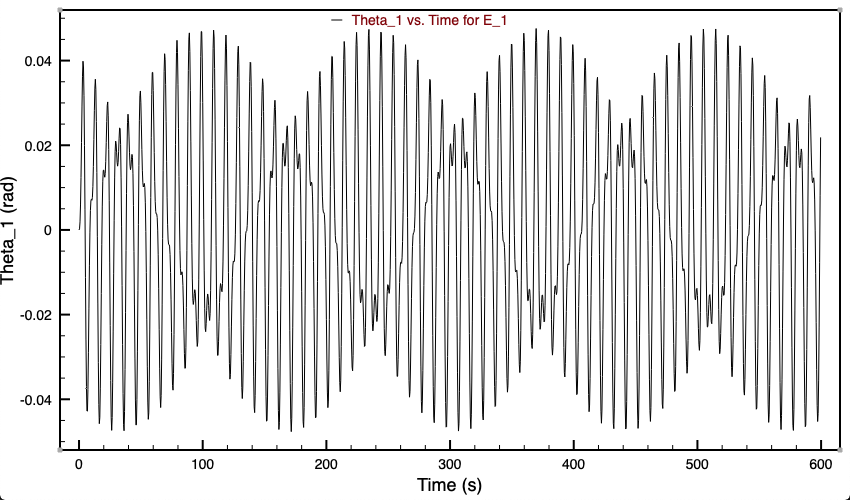
\includegraphics[width=1.\textwidth]{th1vte1.png}
\caption{$\theta_1(t)$ vs. $t$ for $E_1$ with {\tt dt = 0.1} and {\tt tmax = 600}.}
\label{th1vte1}
\end{figure}

\begin{figure}[H]
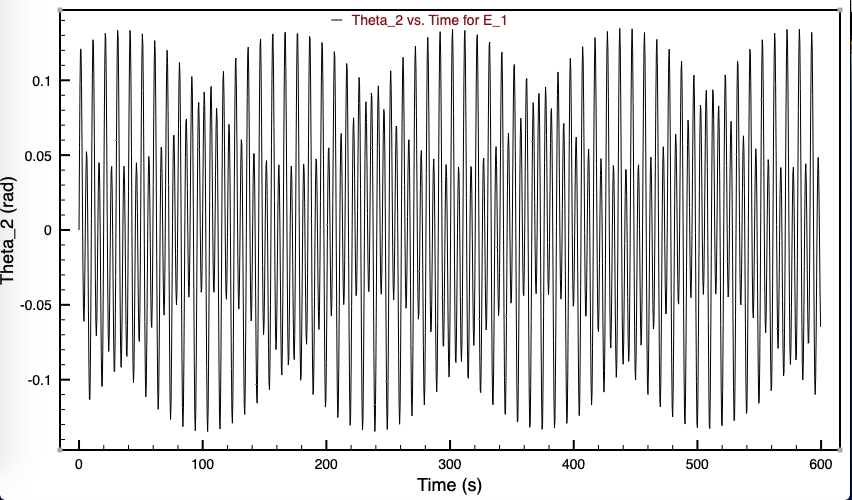
\includegraphics[width=1.\textwidth]{th2vte1.png}
\caption{$\theta_2(t)$ vs. $t$ for $E_1$ with {\tt dt = 0.1} and {\tt tmax = 600}.}
\label{th2vte1}
\end{figure}

\begin{figure}[H]
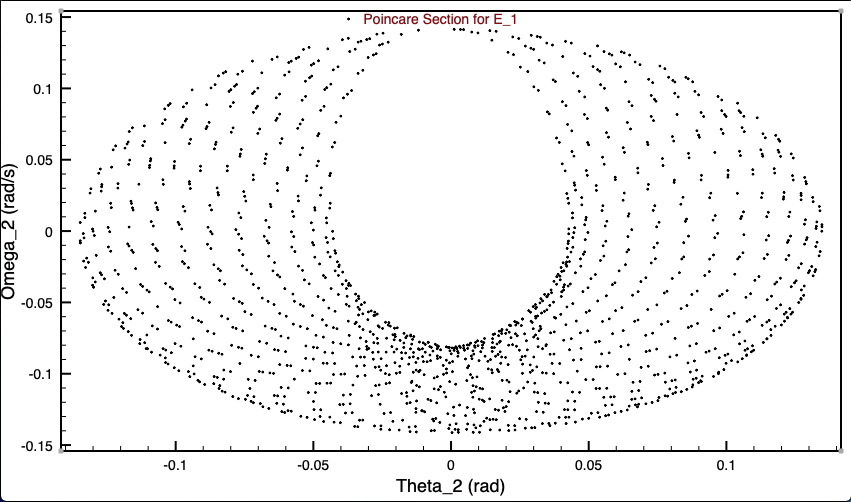
\includegraphics[width=1.\textwidth]{pse1.png}
\caption{Poincare Section for $E_1$ with {\tt dt = 0.1} and {\tt tmax = 600}.}
\label{pse1}
\end{figure}

\begin{figure}[H]
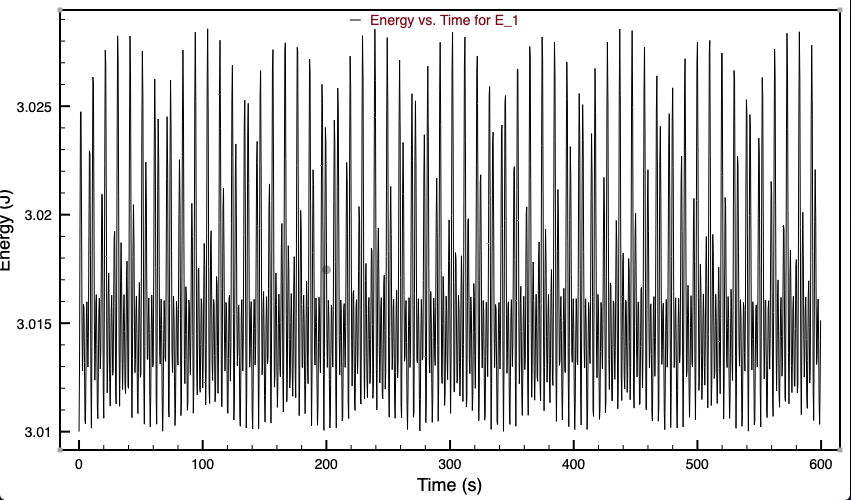
\includegraphics[width=1.\textwidth]{evte1.png}
\caption{Energy vs. $t$ for $E_1$ with {\tt dt = 0.1} and {\tt tmax = 600}.}
\label{evte1}
\end{figure}

\begin{figure}[H]
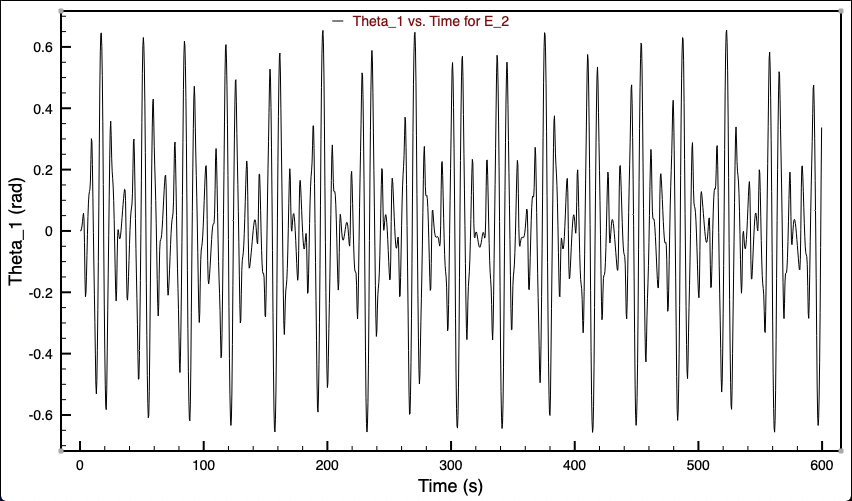
\includegraphics[width=1.\textwidth]{th1vte2.png}
\caption{$\theta_1(t)$ vs. $t$ for $E_2$ with {\tt dt = 0.1} and {\tt tmax = 600}.}
\label{th1vte2}
\end{figure}

\begin{figure}[H]
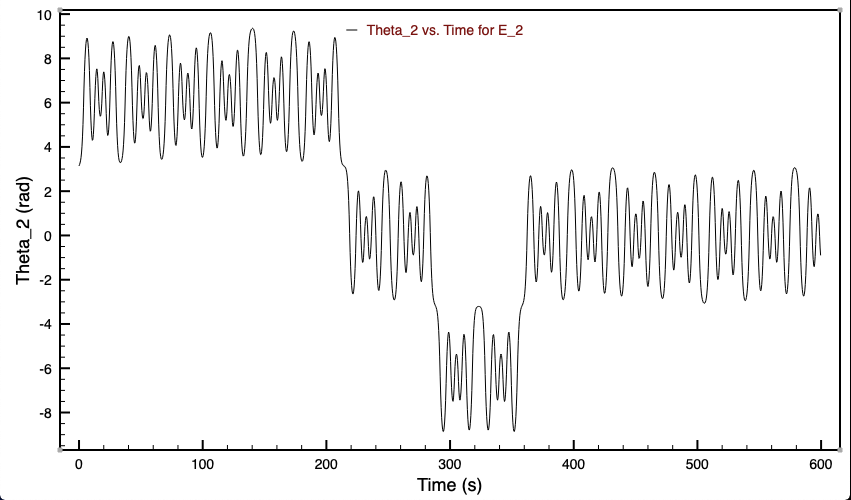
\includegraphics[width=1.\textwidth]{th2vte2.png}
\caption{$\theta_2(t)$ vs. $t$ for $E_2$ with {\tt dt = 0.1} and {\tt tmax = 600}.}
\label{th2vte2}
\end{figure}

\begin{figure}[H]
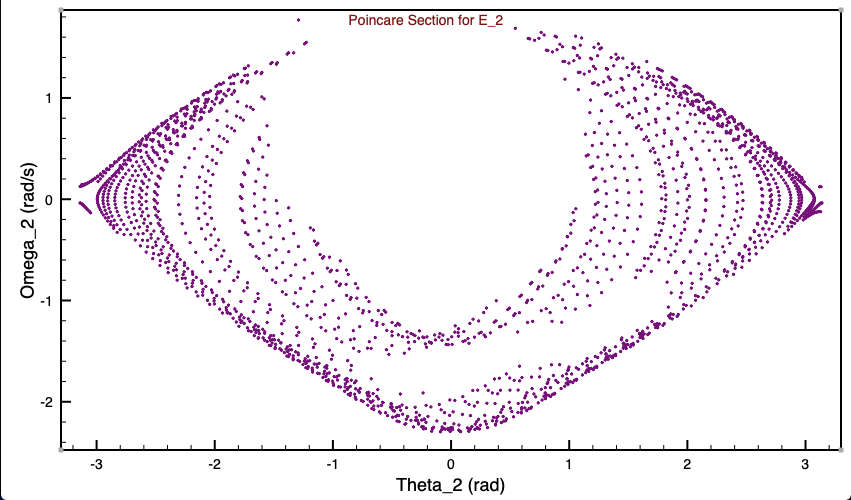
\includegraphics[width=1.\textwidth]{pse2.png}
\caption{Poincare Section for $E_2$ with {\tt dt = 0.1} and {\tt tmax = 600}.}
\label{pse2}
\end{figure}

\begin{figure}[H]
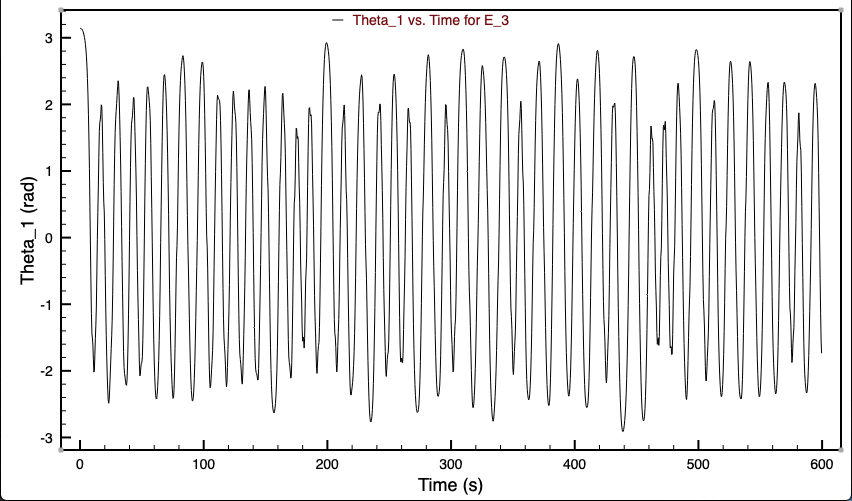
\includegraphics[width=1.\textwidth]{th1vte3.png}
\caption{$\theta_1(t)$ vs. $t$ for $E_3$ with {\tt dt = 0.1} and {\tt tmax = 600}.}
\label{th1vte3}
\end{figure}

\begin{figure}[H]
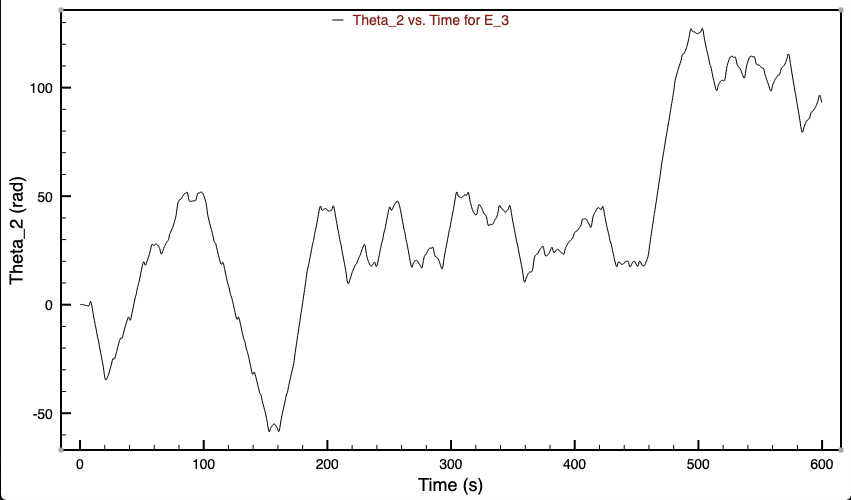
\includegraphics[width=1.\textwidth]{th2vte3.png}
\caption{$\theta_2(t)$ vs. $t$ for $E_3$ with {\tt dt = 0.1} and {\tt tmax = 600}.}
\label{th2vte3}
\end{figure}

\begin{figure}[H]
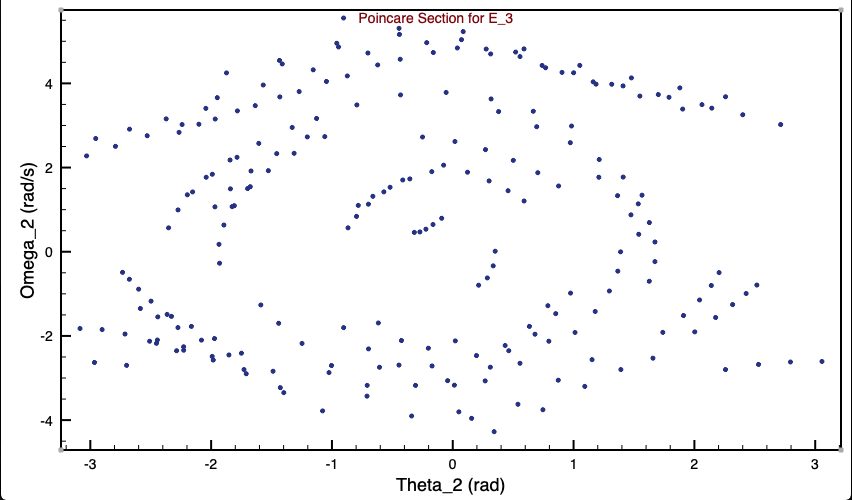
\includegraphics[width=1.\textwidth]{pse3.png}
\caption{Poincare Section for $E_3$ with {\tt dt = 0.1} and {\tt tmax = 600}.}
\label{pse3}
\end{figure}

\begin{figure}[H]
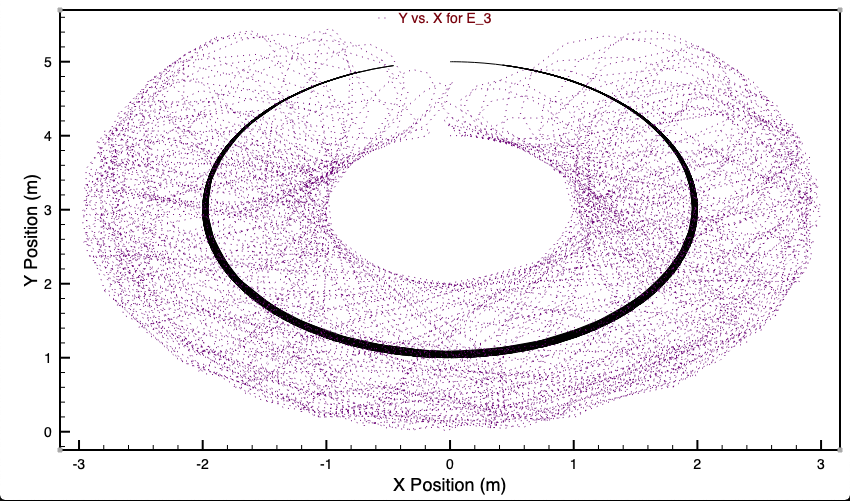
\includegraphics[width=1.\textwidth]{yvxe3.png}
\caption{Spatial path for $E_3$ with {\tt dt = 0.1} and {\tt tmax = 600}.}
\label{yvxe3}
\end{figure}

\begin{figure}[H]
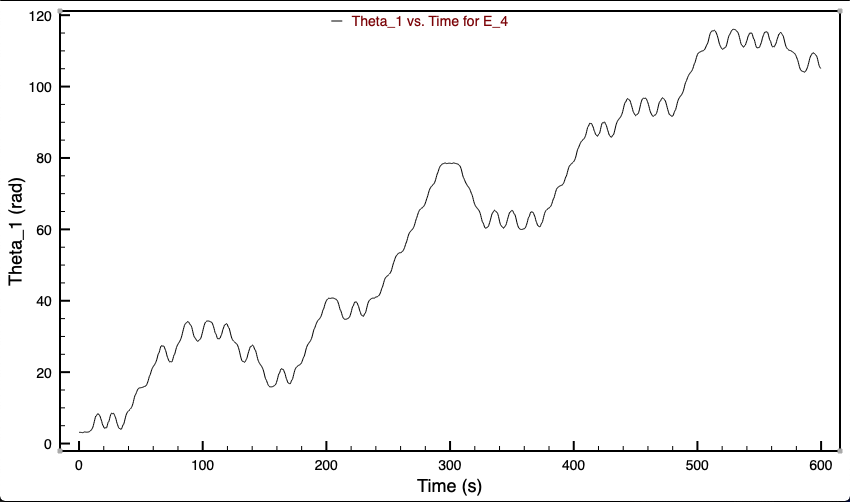
\includegraphics[width=1.\textwidth]{th1vte4.png}
\caption{$\theta_1(t)$ vs. $t$ for $E_4$ with {\tt dt = 0.1} and {\tt tmax = 600}.}
\label{th1vte4}
\end{figure}

\begin{figure}[H]
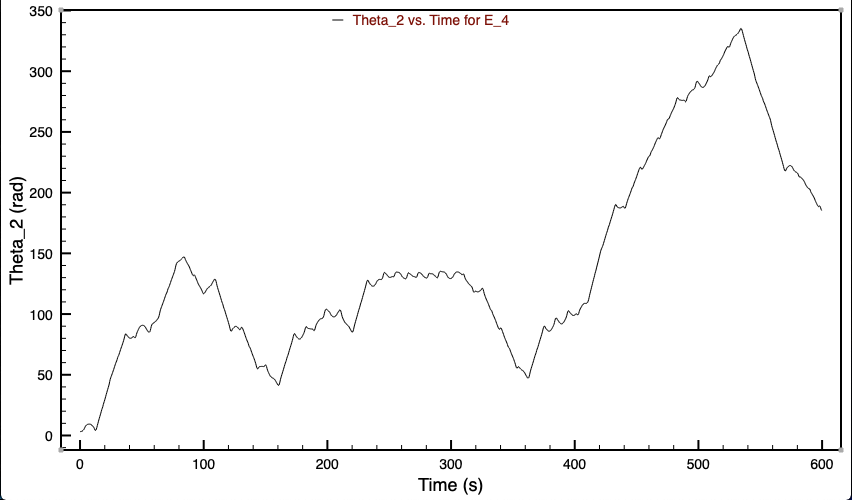
\includegraphics[width=1.\textwidth]{th2vte4.png}
\caption{$\theta_2(t)$ vs. $t$ for $E_4$ with {\tt dt = 0.1} and {\tt tmax = 600}.}
\label{th2vte4}
\end{figure}

\begin{figure}[H]
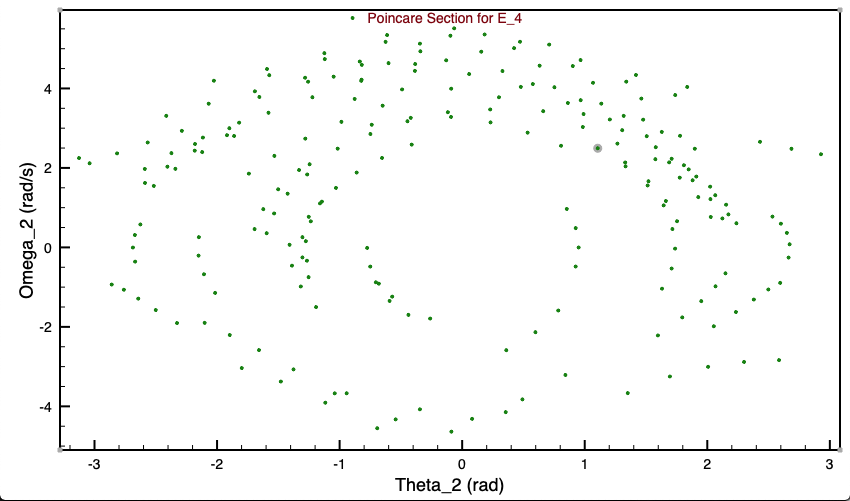
\includegraphics[width=1.\textwidth]{pse4.png}
\caption{Poincare Section for $E_4$ with {\tt dt = 0.1} and {\tt tmax = 600}.}
\label{pse4}
\end{figure}

\section{Problem 2}

For problem 2 we are given a neutron star that is vibrating and are tasked to show that the z-component of its spin, $\Omega (t)$, is nearly constant while the vector $\Omega(t)$ nutates abput the $z$-axis. We are given the oscillating moments of inertia:

\[I_{zz} = I_0(1+\epsilon cos(\omega t))\]
\[I_{xx} = I_{yy} = I_0(1-\frac{\epsilon}{2}cos(\omega t)), \epsilon << 1, I_0=\frac{2}{5}mr^2.\]

We can take advantage of the Euler equations for the body-fixed system \cite{greiner}:

\[N = \dot{L}+\Omega \times L\]

$N$ is equal to zero for this system since there are no external forces.  This yields the equations of motion (for $g=\epsilon cos(\omega t)$):


\[\dot{L_x} = \frac{-3 L_y L_z g}{2 I_0 (1+g)(1-\frac{g}{2})}\]
\[\dot{L_y} = \frac{3 L_x L_z g}{2 I_0 (1+g)(1-\frac{g}{2})}\]
\[\dot{L_z} = 0\]

The code is found in Listing \ref{starvibe}.  The {\tt numtype} module is identical to the one used before in Listing \ref{numtype}.  The {\tt Makefile} is very similar, with the only differences being contained in Listing \ref{makefile2}.  This gives instructions for the compiler when typing {\tt make} into the terminal.  The code can then be executed by typing {\tt star}.  The program {\tt starvibe} begins with the module {\tt setup} which inputs the parameters for the problem.  For our calculation of $I_0$, the value $\epsilon =10^{-8}$ was chosen.  The time parameters can be inputted, in this case the graphs are plotted for a time of 20 s with  {\tt dt=0.01}.  The elements of the vector y(1:3) exist so that the length of the arrays $y$ and $f$ are equal.  The equations of motion above represent a coupled first-order differential equation for the angular momentum $L$.  $y(4:6)$ are the $x$, $y$, and $z$-components respectively of the angular momentum vector $L$.  The elements of the array $f(1:3)=y(4:6)$ and its derivatives are $f(4:6)$.  \emph{rk4} was used instead of \emph{rkf45} because the adaptive-step size kept going to 0.  Since we were given a magnitude for $\Omega(t)$, it was evenly split between its three components.  Since the $y$ array is in terms of the angular momentum, $O$ is used to divide by the moments of inertia to get the components of the angular velocity, which are to be graphed.  The files {\tt fort.1}, {\tt fort.2} and {\tt fort.3} are the files written for the $x$, $y$ and $z$-components of the angular momentum respectively vs. time.  The three are plotted on the same graph in Fig. \ref{prob2}.  \textbf{This graph shows that the $z$-component of $\Omega$ remains nearly constant, and the sinusoidal nature of the plots for $\Omega_x$ and $\Omega_y$ show that $\Omega(t)$ nutates about the z-axis with nutation frequency approximately 0.3 Hz.}

\begin{lstlisting}[frame=single,caption={Module {\tt numtype}},label=makefile2]

objs1 = numtype.o starvibe.o rkf45step.o

prog1 = star

\end{lstlisting}

\begin{lstlisting}[frame=single,caption={Module {\tt numtype}},label=starvibe]

module setup

    use numtype
    implicit none
    integer, parameter :: n_eq = 6

    real(dp), parameter :: m = 40.e30_dp, &
        r = 10.e3_dp, nu = 40.e3_dp, eps = 10.e-8_dp

end module setup

program starvibe

    use setup
    implicit none
    real(dp), dimension(n_eq) :: y
    real(dp), dimension(3) :: O
    real(dp) :: t, dt, tmax, omega, w, I0, &
        Ix, Iy, Iz
    integer :: i

    t = 0._dp
    dt = 0.01_dp
    tmax = 20._dp

    w = 2 * pi * nu
    omega = 100 * w
    I0 = 2._dp / 5 * m * r**2

    y(1) = 0._dp
    y(2) = 0._dp
    y(3) = 0._dp
    y(4) = I0 * omega / sqrt(3._dp) ! L_x
    y(5) = I0 * omega / sqrt(3._dp) ! L_y
    y(6) = I0 * omega / sqrt(3._dp) ! L_z

    do while ( t < tmax )

        Ix = I0 * ( 1 - eps / 2 * cos( w * t ) )
        Iy = Ix
        Iz = I0 * ( 1 + eps * cos( w * t ) )

        O(1) = y(4) / Ix 
        O(2) = y(5) / Iy 
        O(3) = y(6) / Iz

        do i = 1 , 3
            write(i,*) t, O(i)
        end do

        call rk4step( t, dt, y )

    end do

end program starvibe

subroutine rk4step(x, h, y)

    use setup
    implicit none
    real(dp), intent(inout) :: x
    real(dp), intent(in) :: h
    real(dp), intent(inout), dimension(n_eq) :: y
    real(dp), dimension(n_eq) :: k1, k2, k3, k4, dy

    k1 = kv (x, h, y)
    k2 = kv (x+h/2, h, y+k1/2)
    k3 = kv (x+h/2, h, y+k2/2)
    k4 = kv (x+h, h, y+k3)

    dy = (k1 + 2*k2 + 2*k3 + k4) / 6

    x = x + h 
    y = y + dy

    contains

        function kv (t, dt, y) result(k)

            use setup
            implicit none
            real(dp), intent(in) :: t
            real(dp), intent(in) :: dt
            real(dp), intent(in), dimension(n_eq) :: y
            real(dp), dimension(n_eq) :: f, k
            real(dp) :: I0, w, g

            I0 = 2._dp / 5 * m * r**2
			w = 2 * pi * nu
			g = eps * cos ( w * t )

	        f(1:3) = y(4:6)

			f(4) = - 3 / ( 2 * I0 ) * y(5) * y(6) &
			    & * g / ( ( 1 + g ) * ( 1 - g / 2 ) )

			f(5) = 3 / ( 2 * I0 ) * y(4) * y(6) &
			    & * g / ( ( 1 + g ) * ( 1 - g / 2 ) )

			f(6) = 0

            k(1:n_eq) = h*f(1:n_eq)

        end function kv

end subroutine rk4step

\end{lstlisting}

\begin{figure}[H]
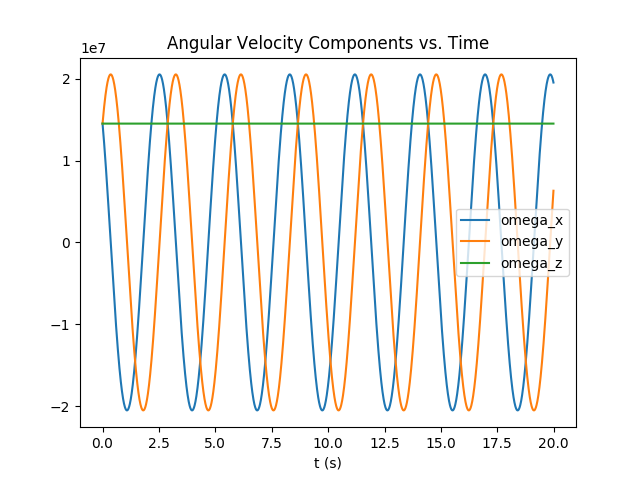
\includegraphics[width=1.\textwidth]{prob2.png}
\caption{Components of angular velocity with respect to time for {\tt dt = 0.01} and {\tt tmax = 20}.}
\label{prob2}
\end{figure}

\section{Summary and conclusions}

We presented our {\tt Fortran90} codes for the solutions of Problem 1 and 2 from Midterm 1.  We can see that the motion for a double pendulum is approximately harmonic for $\theta_1 \approx 0$, but as $\theta_1$ increases the behavior becomes more chaotic.  We also observed that a neutron star with the given vibrating moments of inertia will maintain a nearly-constant $\Omega_z$ while nutating about the z-axis.  Ultimately, we have been shown the incredible power of the Runge-Kutta method, specifically RK4, for allowing us to study interesting physics with simulations of nonlinear phenomena that could otherwise not be solved for analytically.

\begin{thebibliography}{}

\bibitem{wiki} Runge-Kutta methods. (n.d.). In {\it Wikipedia}. Retrieved March 3, 2020, from https://en.wikipedia.org/wiki/Runge–Kutta\_methods

\bibitem{weisstein} Weisstein, Eric W. "Runge-Kutta Method." From {\it MathWorld}--A Wolfram Web Resource.\\ 
http://mathworld.wolfram.com/Runge-KuttaMethod.html

\bibitem{neumann} Neumann, Erik "Double Pendulum." In {\it myPhysicsLab}. Retrieved March 4, 2020, from http://mathworld.wolfram.com/Runge-KuttaMethod.html

\bibitem{greiner} Greiner, W. (2009). \emph{Classical Mechanics: systems of particles and Hamiltonian dynamics}. Springer Science \& Business Media.
 
\end{thebibliography}

\end{document}
